% RQ4 Results: Treasury Resilience

\subsection{Overview}

We present results from \experimentruns{} simulation runs across 12 treasury policy configurations.

\begin{table}[htbp]
\centering
\caption{RQ4 Results Overview (Experiment 06)}
\label{tab:rq4-overview}
\begin{tabular}{lr}
\toprule
Parameter & Value \\
\midrule
Policy configurations & 12 \\
Runs per configuration & 25 \\
Total simulation runs & 300 \\
\bottomrule
\end{tabular}
\end{table}

\subsection{Buffer Fraction Effects}

\subsubsection{Volatility Reduction}

\begin{figure}[htbp]
    \centering
    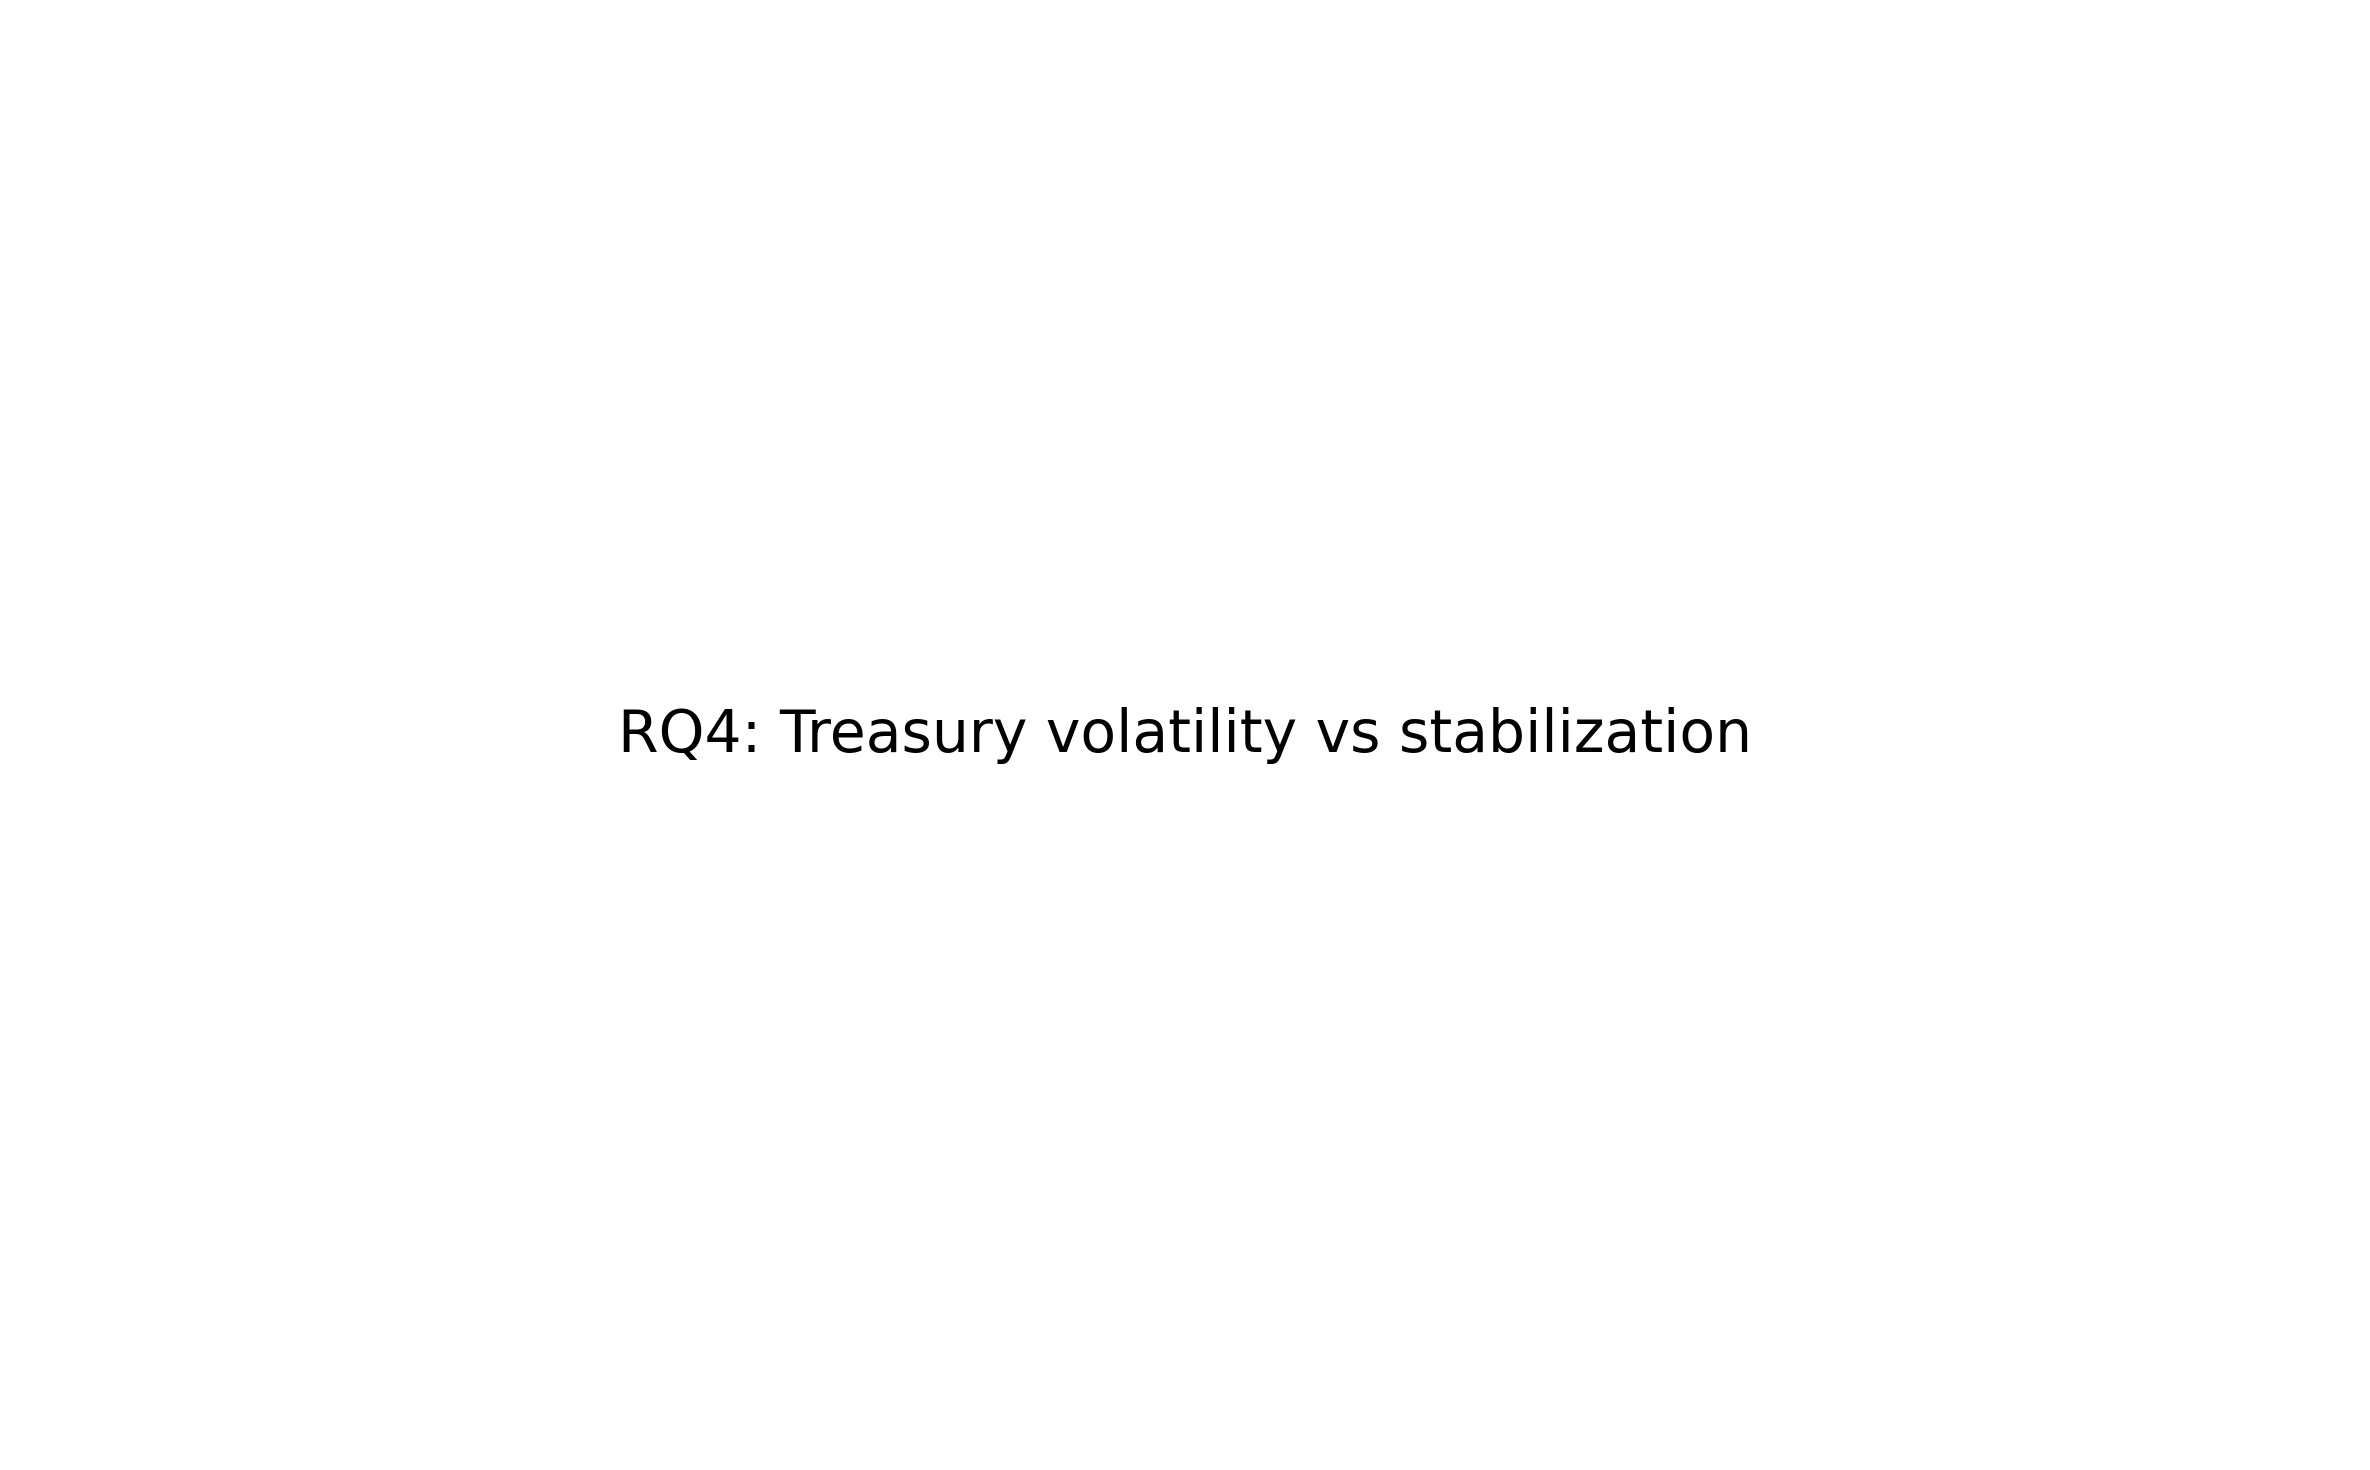
\includegraphics[width=0.8\textwidth]{../figures/rq4_volatility}
    \caption{Treasury volatility (standard deviation) by buffer fraction. Higher buffers substantially reduce volatility, with diminishing returns above 20\%.}
    \label{fig:rq4-volatility}
\end{figure}

\begin{table}[htbp]
\centering
\caption{Volatility and drawdown by buffer fraction}
\label{tab:rq4-buffer}
\begin{tabular}{lccc}
\toprule
Buffer & Volatility & Max Drawdown & Final Treasury \\
\midrule
\pl{0\%} & \pl{--} & \pl{--} & \pl{--} \\
\pl{10\%} & \pl{--} & \pl{--} & \pl{--} \\
\pl{20\%} & \pl{--} & \pl{--} & \pl{--} \\
\pl{30\%} & \pl{--} & \pl{--} & \pl{--} \\
\bottomrule
\end{tabular}
\end{table}

\subsubsection{Efficiency Tradeoff}

\begin{figure}[htbp]
    \centering
    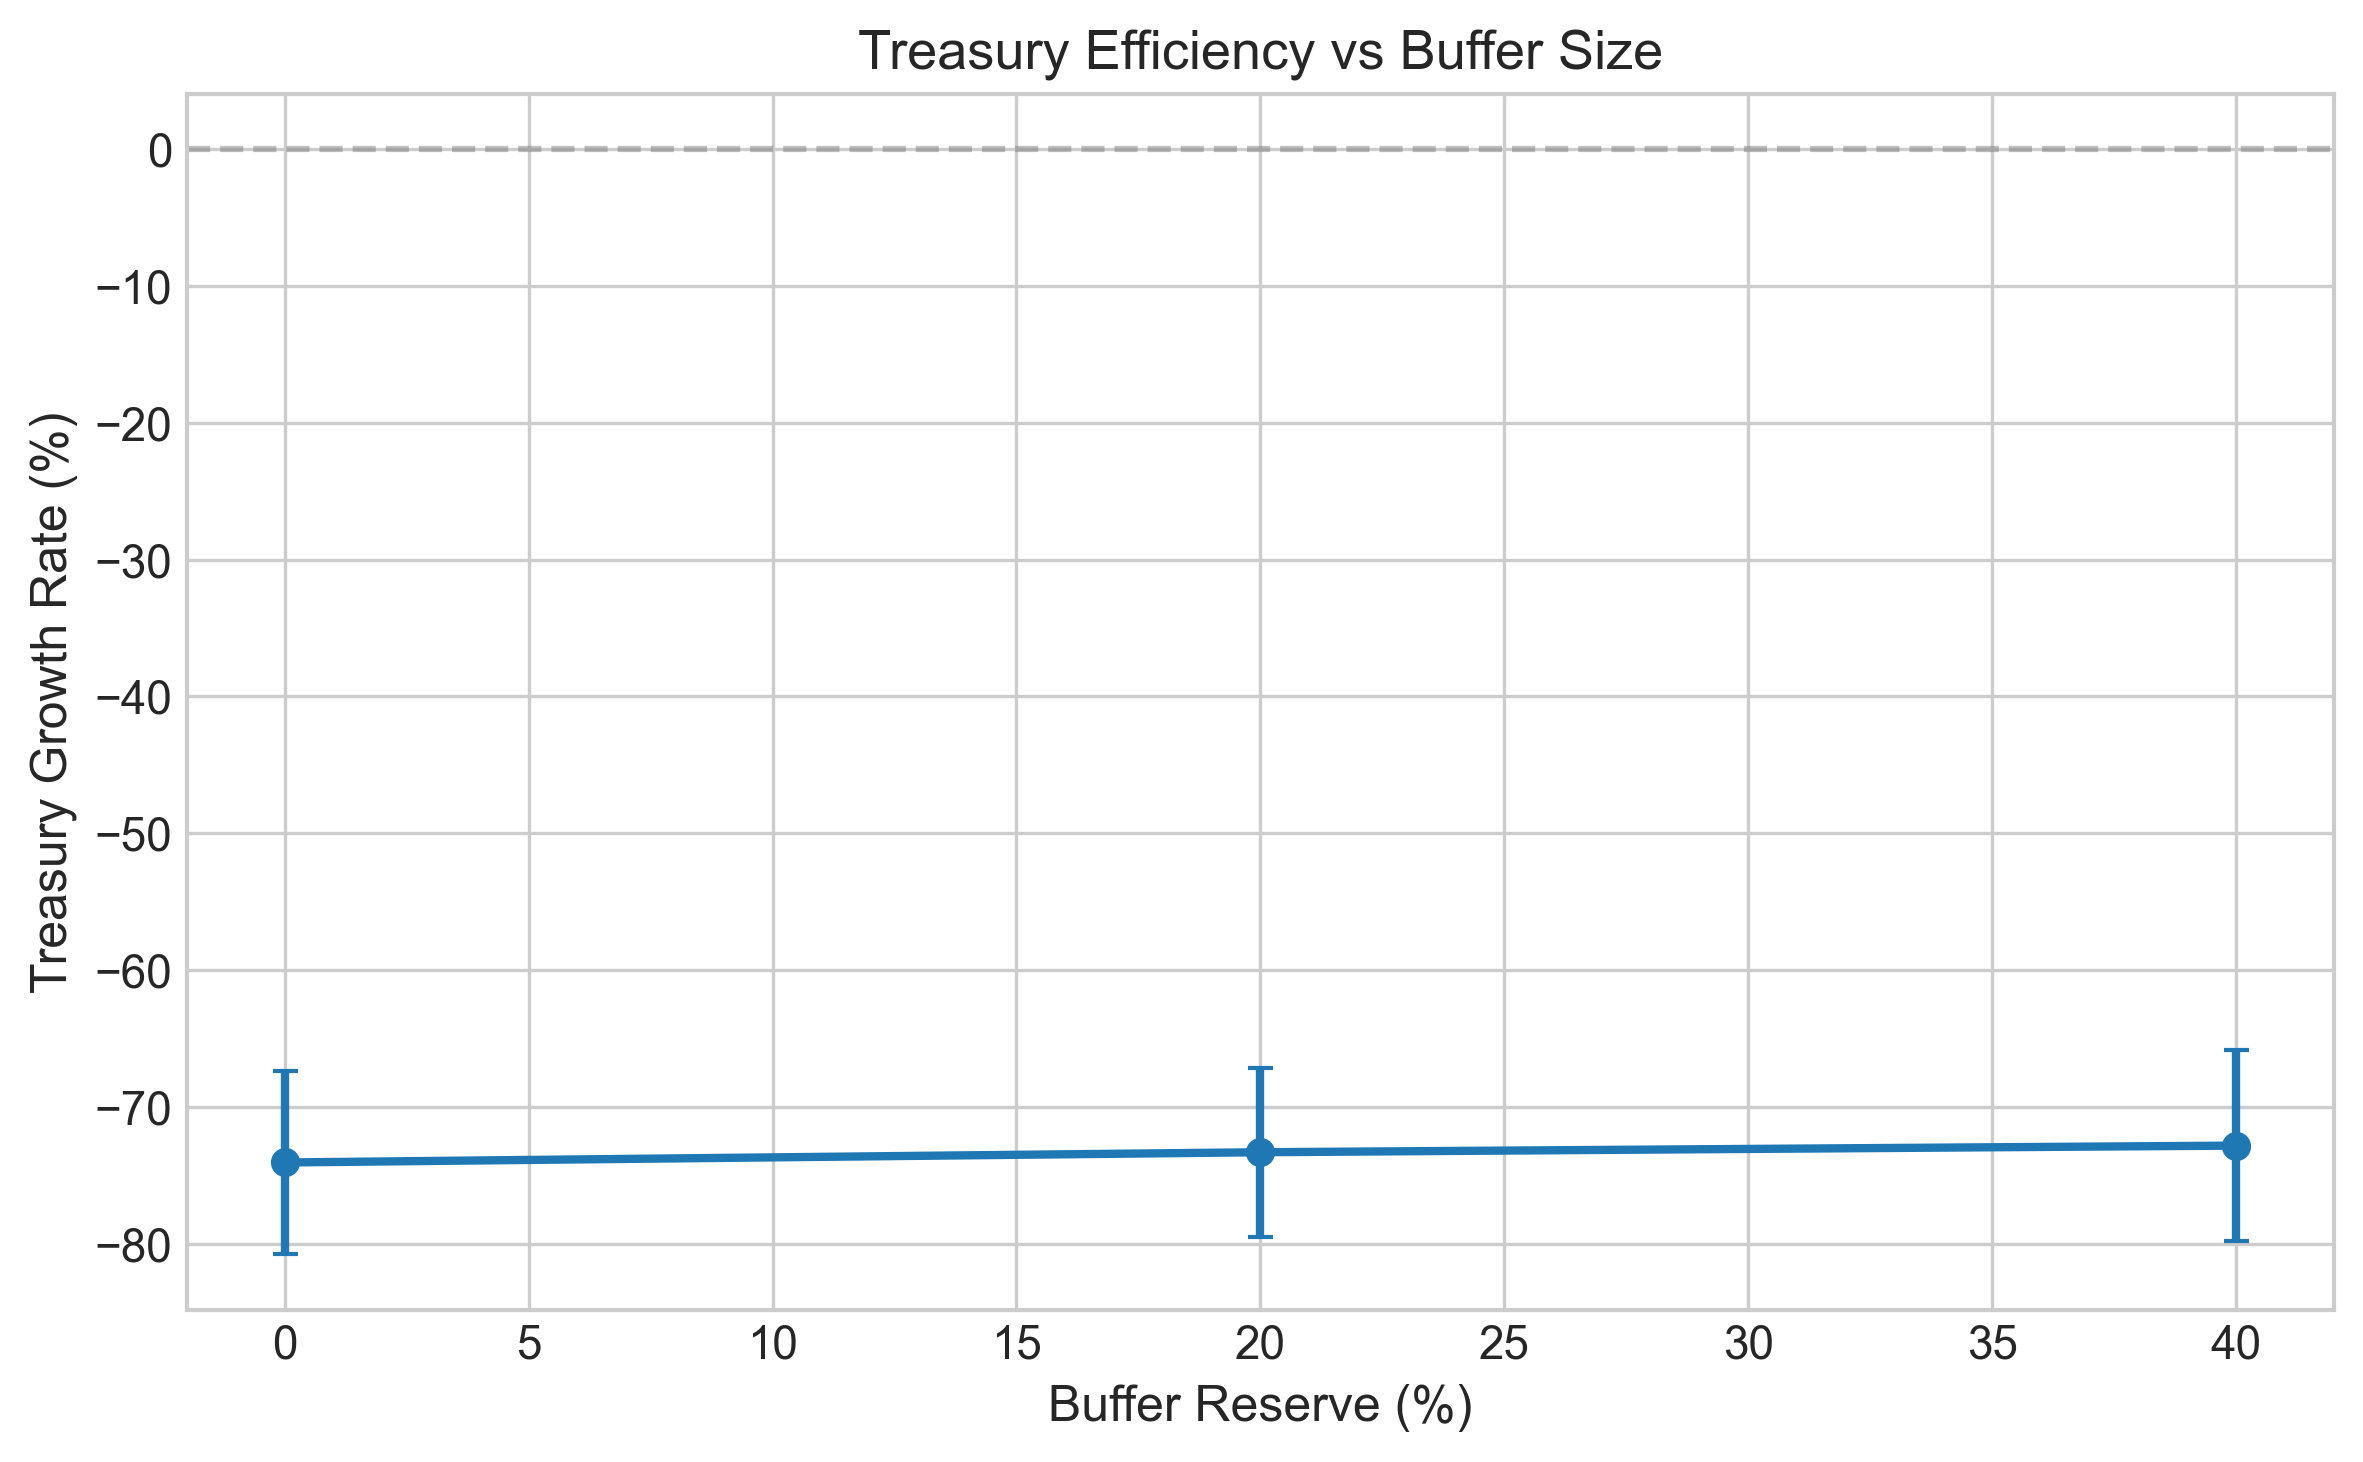
\includegraphics[width=0.8\textwidth]{../figures/rq4_efficiency}
    \caption{Proposal throughput (proposals funded) vs. buffer fraction. Larger buffers reduce available spending, constraining proposal funding.}
    \label{fig:rq4-efficiency}
\end{figure}

\subsection{Spending Limit Effects}

\subsubsection{Runway Extension}

\begin{figure}[htbp]
    \centering
    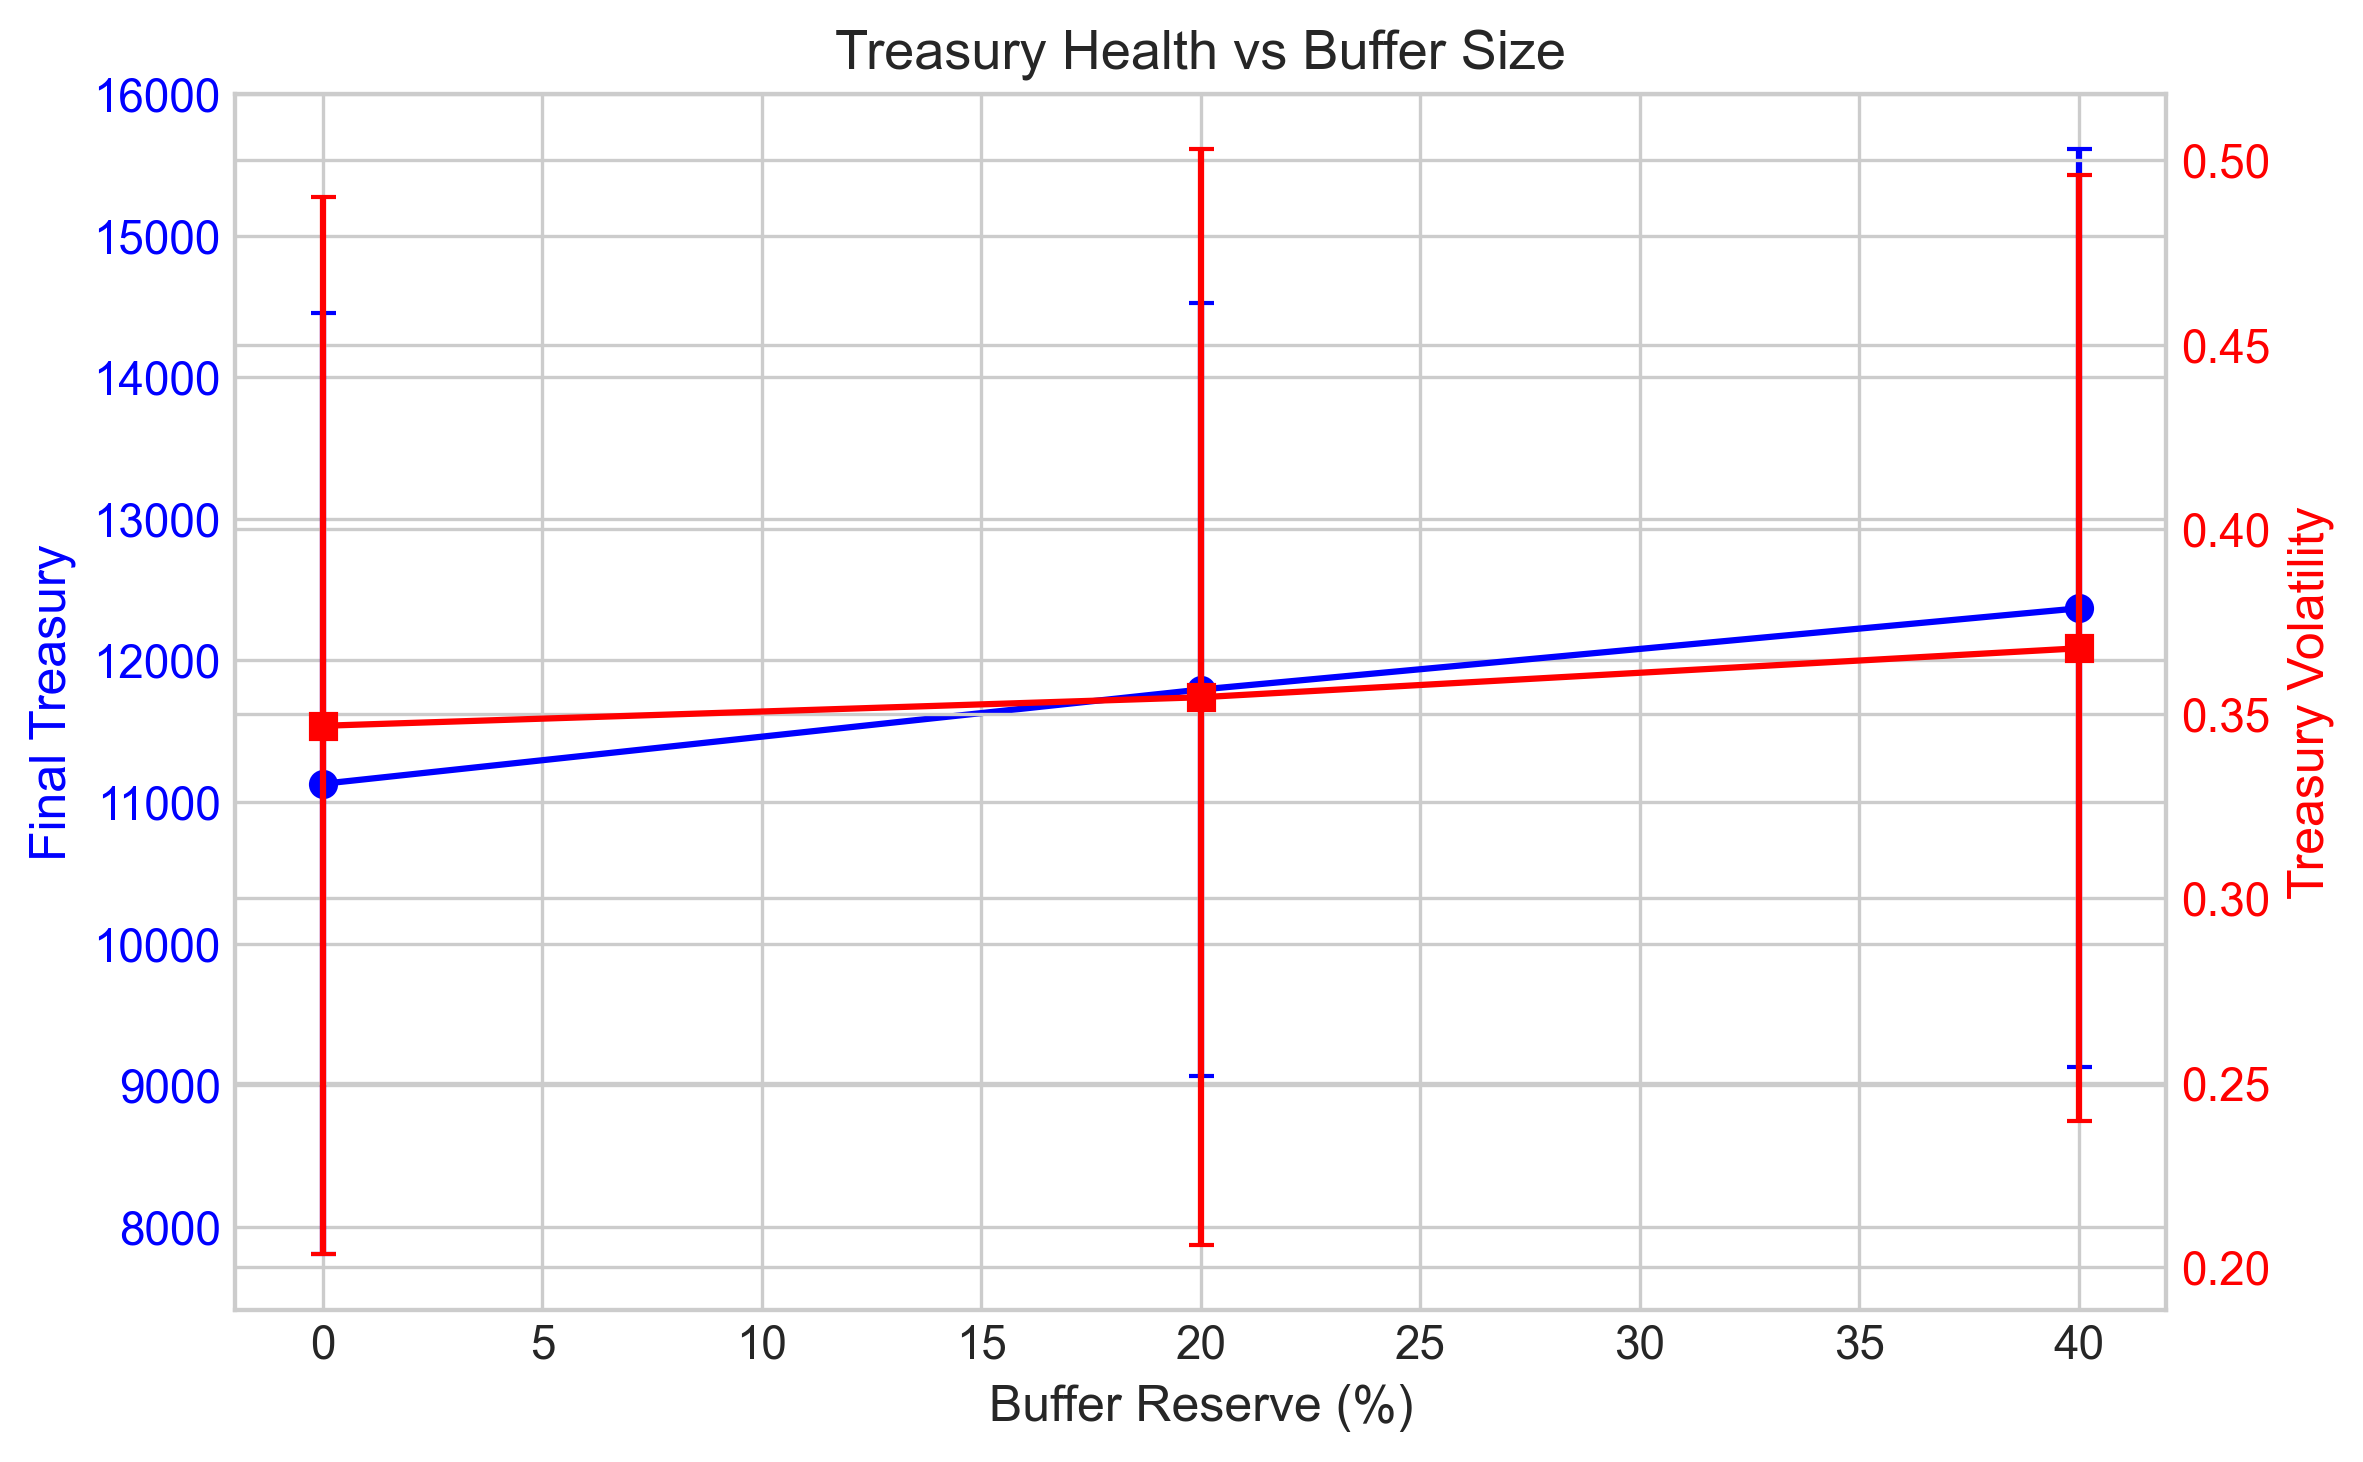
\includegraphics[width=0.8\textwidth]{../figures/rq4_runway}
    \caption{Treasury runway (steps until depletion) by spending limit. Tighter limits extend runway but may cause funding backlogs.}
    \label{fig:rq4-runway}
\end{figure}

\begin{table}[htbp]
\centering
\caption{Runway and throughput by spending limit}
\label{tab:rq4-limits}
\begin{tabular}{lccc}
\toprule
Limit & Runway & Proposal Throughput & Funding Backlog \\
\midrule
\pl{None} & \pl{--} & \pl{--} & \pl{--} \\
\pl{5\%} & \pl{--} & \pl{--} & \pl{--} \\
\pl{2\%} & \pl{--} & \pl{--} & \pl{--} \\
\bottomrule
\end{tabular}
\end{table}

\subsection{Emergency Top-Up Effects}

\subsubsection{Drawdown Mitigation}

\begin{figure}[htbp]
    \centering
    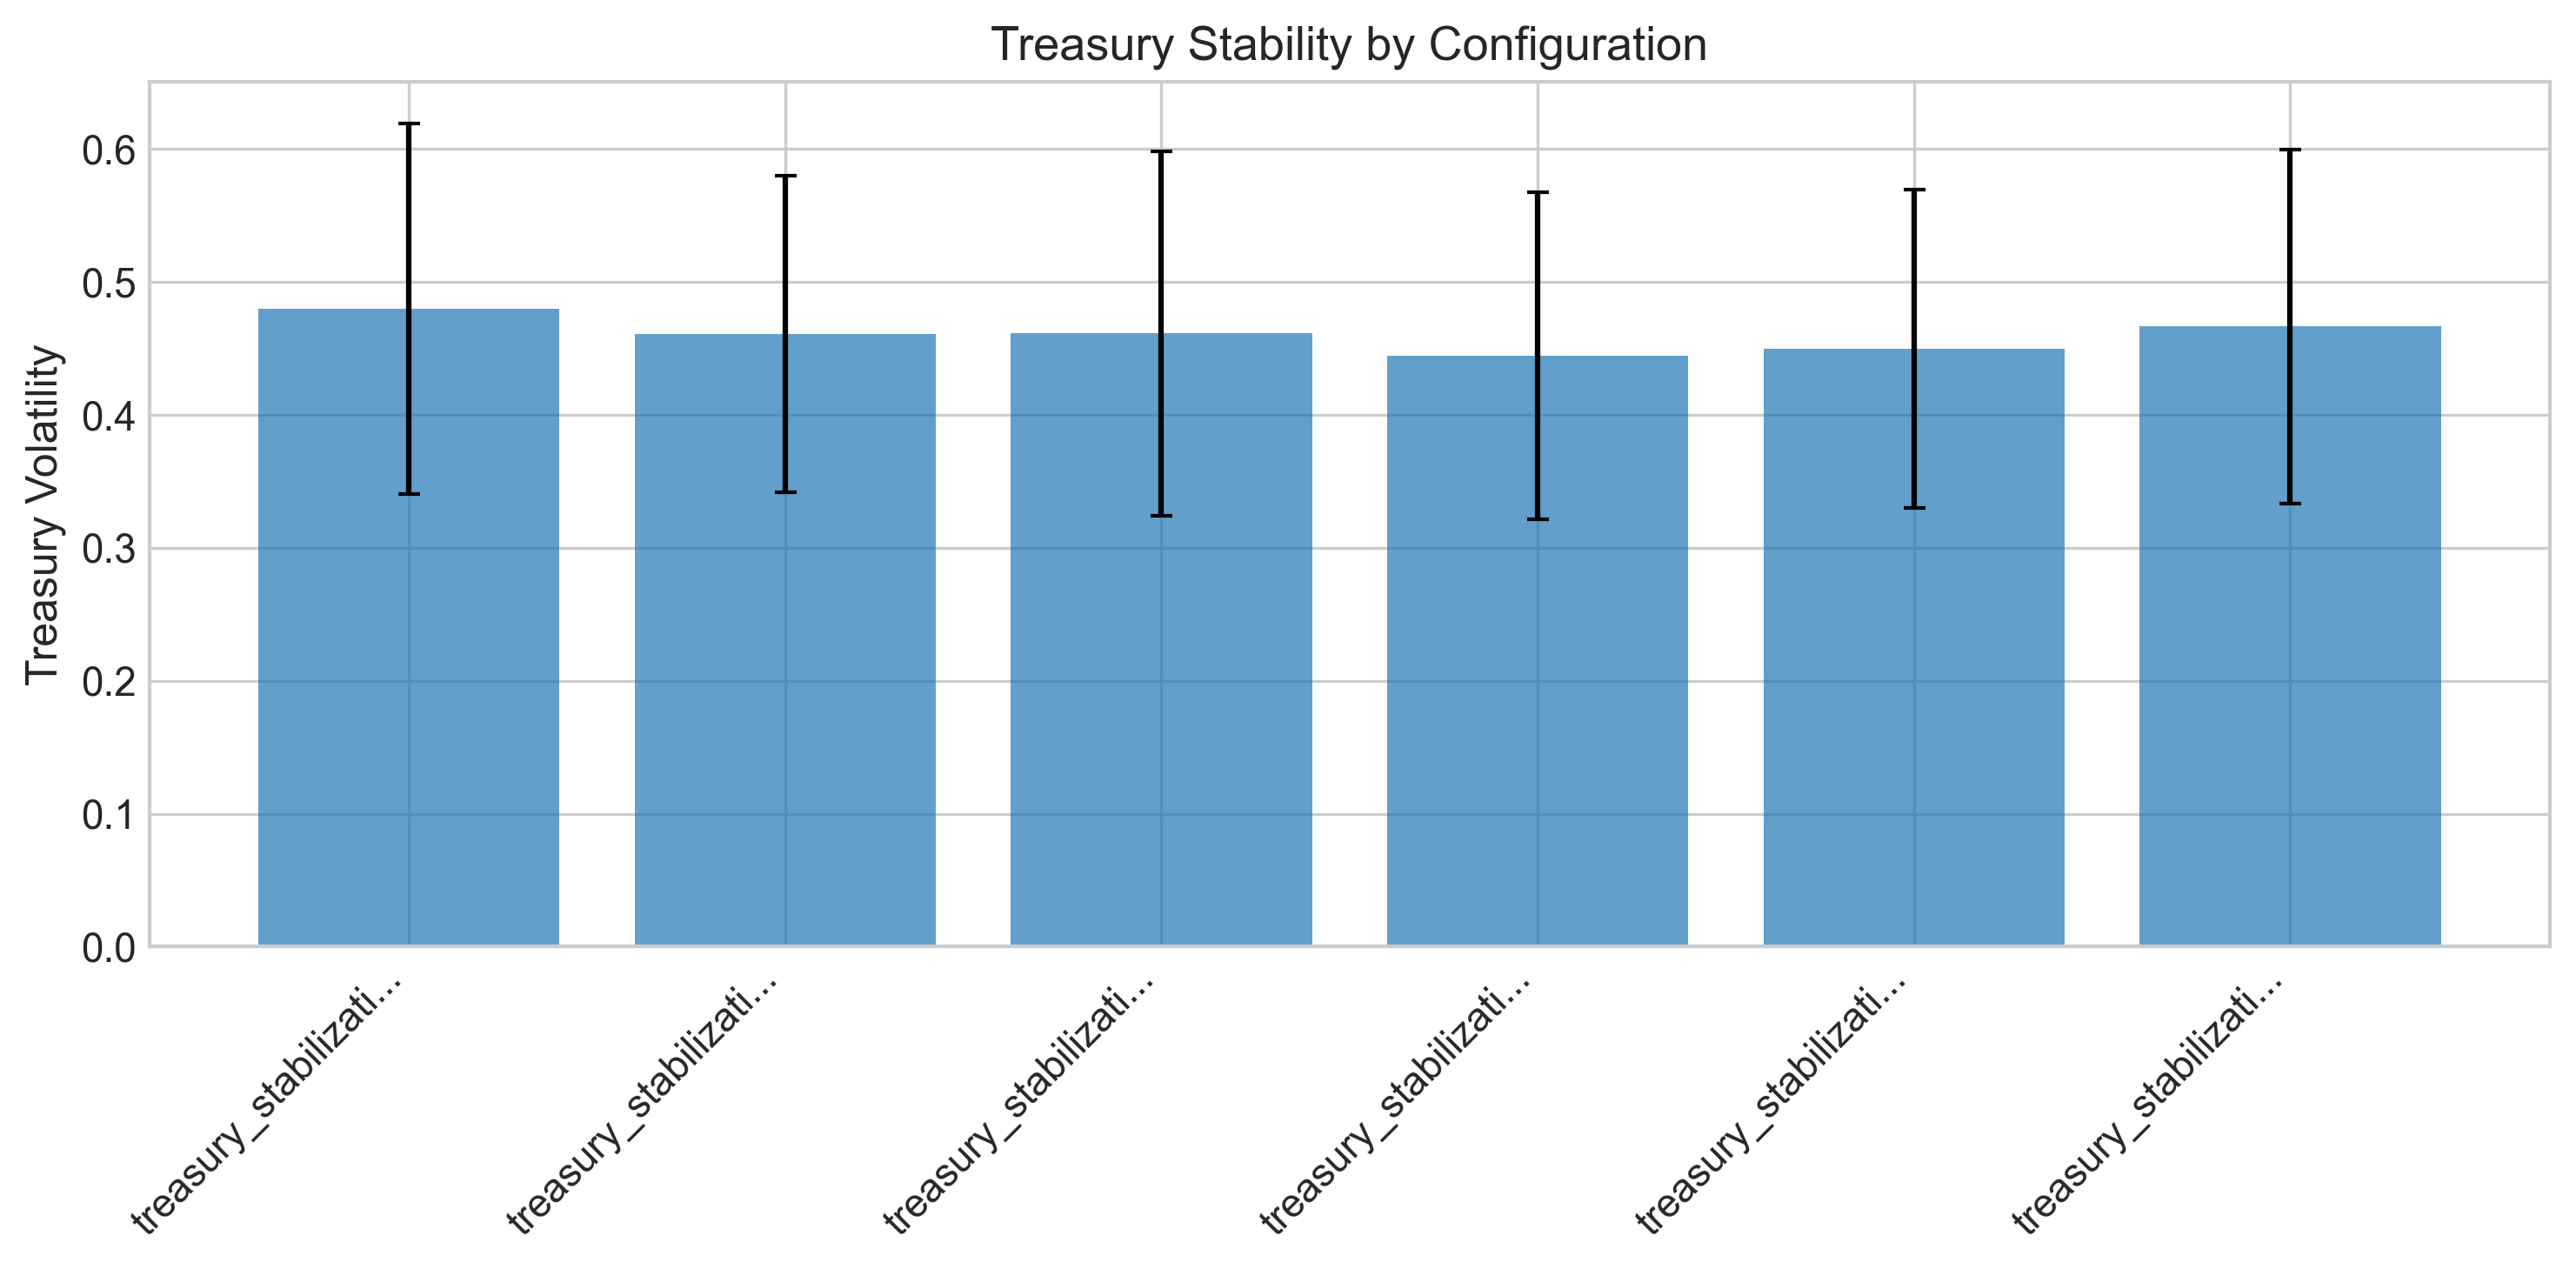
\includegraphics[width=0.8\textwidth]{../figures/rq4_topup}
    \caption{Maximum drawdown by top-up mode. Both revenue diversion and spending freeze reduce drawdown severity.}
    \label{fig:rq4-topup}
\end{figure}

\begin{table}[htbp]
\centering
\caption{Top-up mechanism effectiveness}
\label{tab:rq4-topup}
\begin{tabular}{lccc}
\toprule
Top-Up Mode & Max Drawdown & Recovery Time & Throughput Impact \\
\midrule
\pl{None} & \pl{--} & \pl{--} & \pl{--} \\
\pl{Revenue divert} & \pl{--} & \pl{--} & \pl{--} \\
\pl{Spending freeze} & \pl{--} & \pl{--} & \pl{--} \\
\bottomrule
\end{tabular}
\end{table}

\subsection{Market Regime Interactions}

\begin{figure}[htbp]
    \centering
    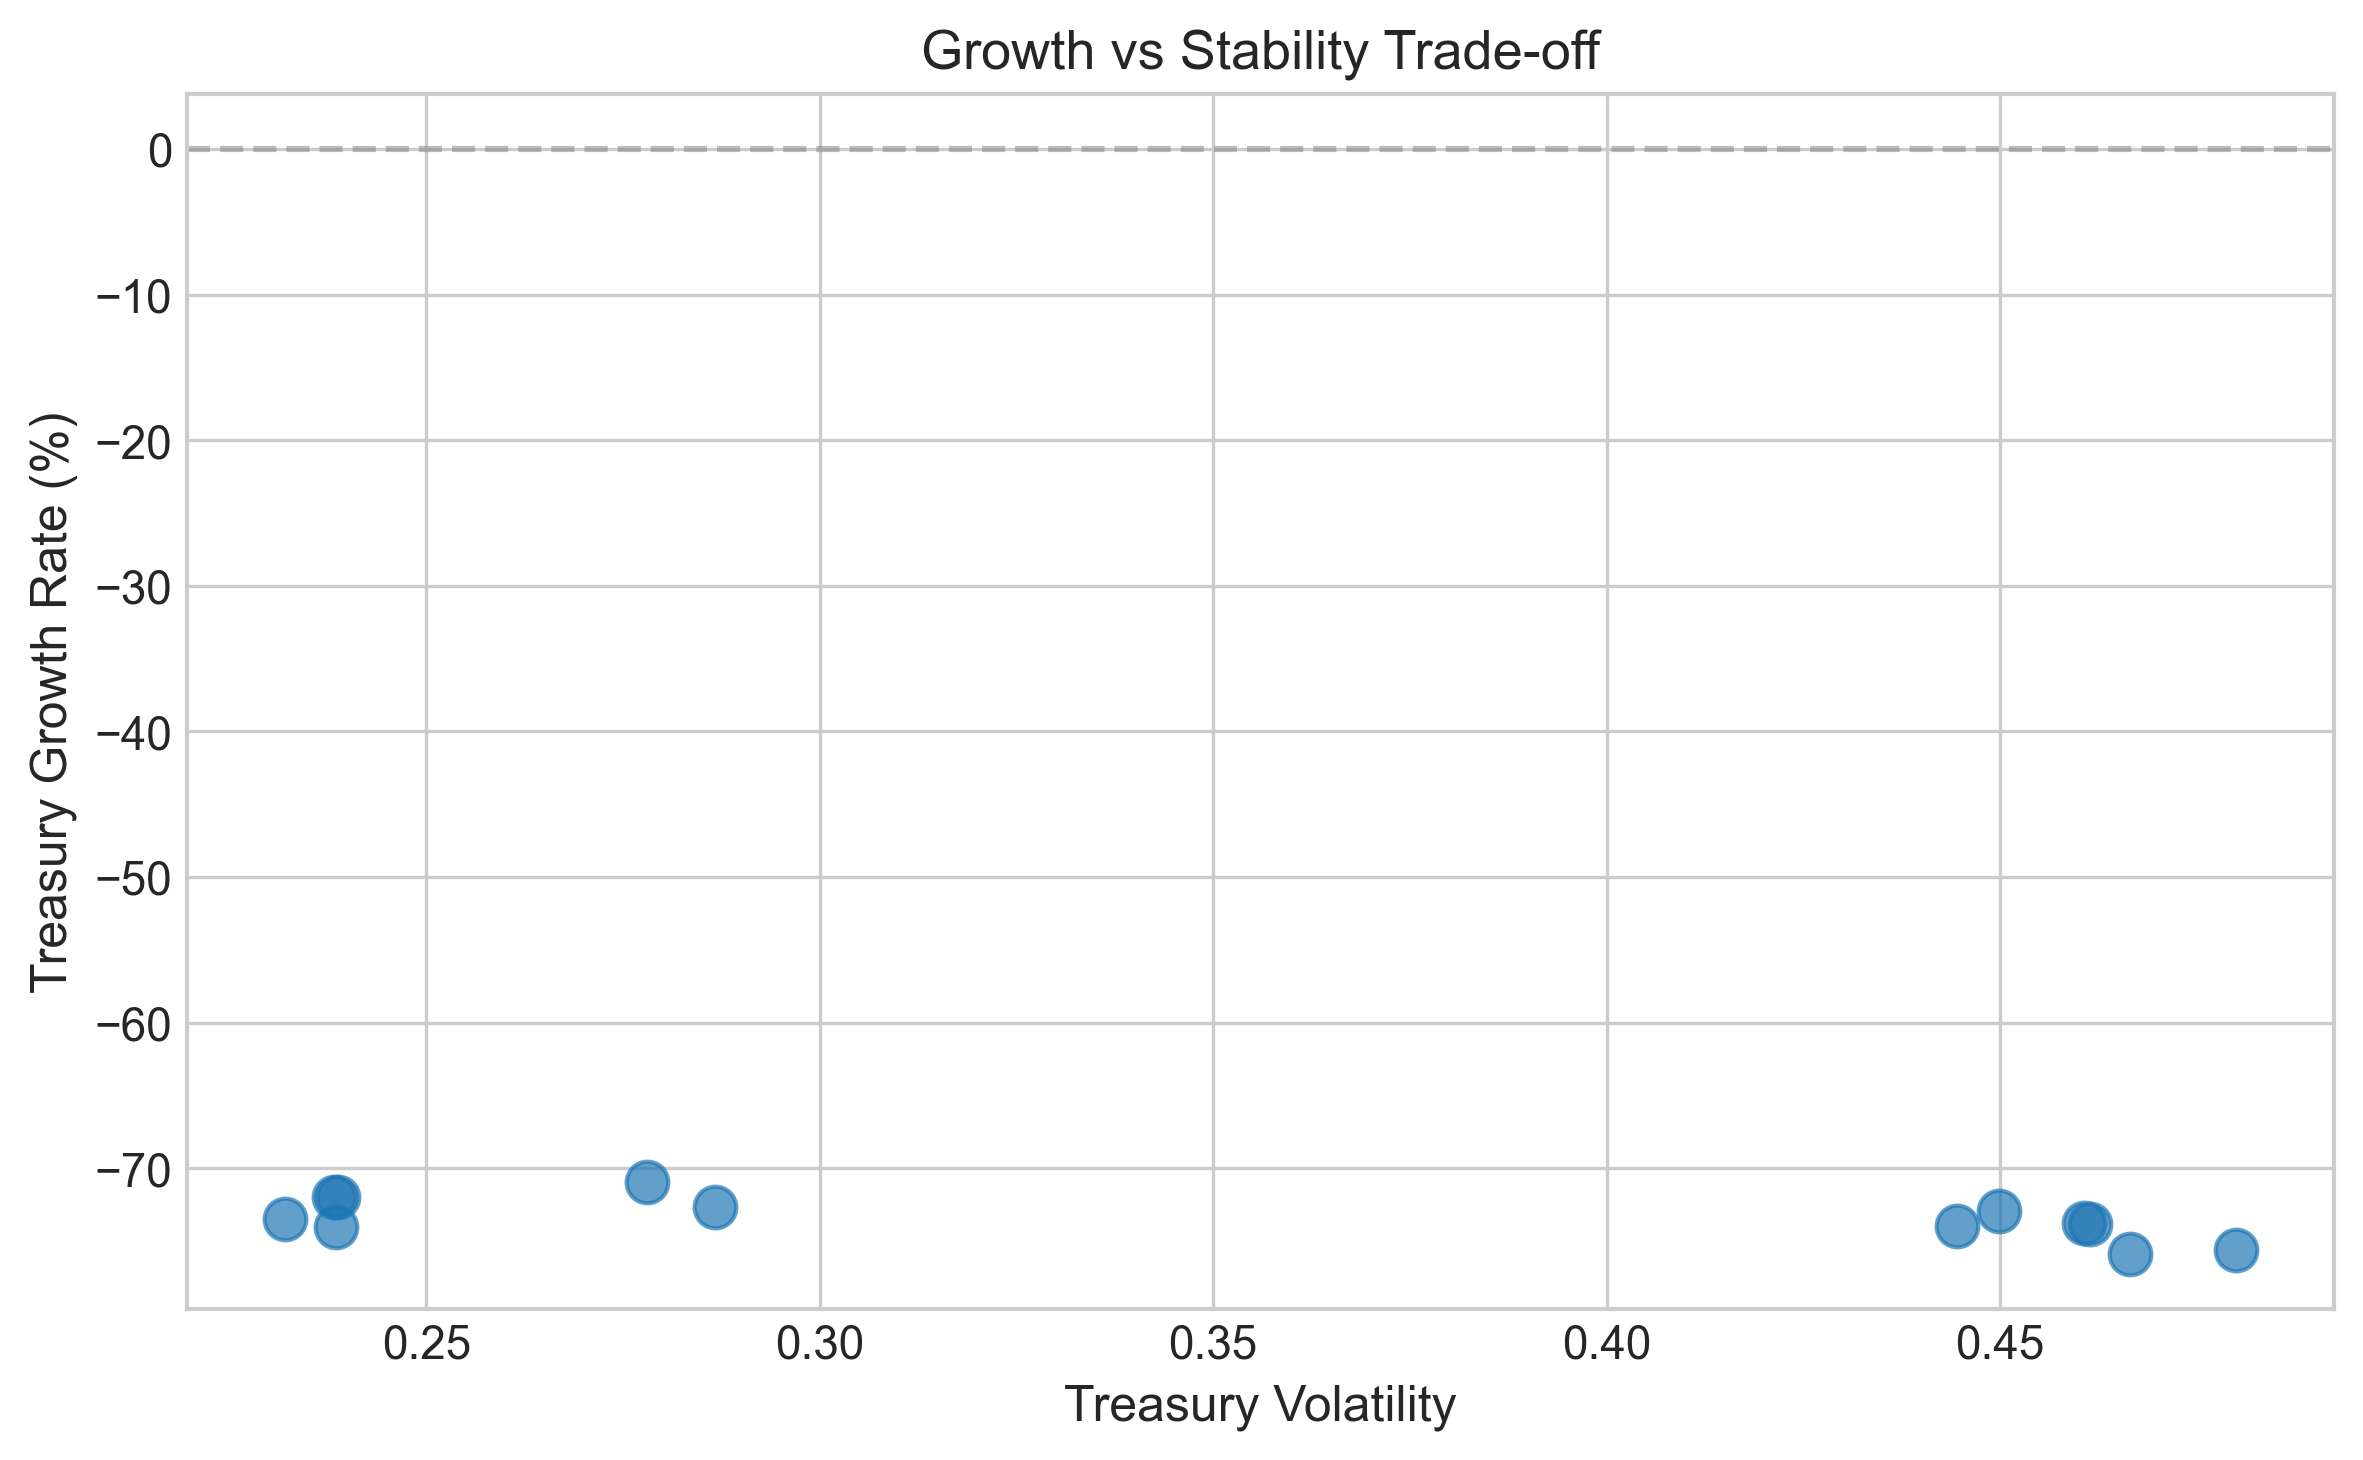
\includegraphics[width=0.8\textwidth]{../figures/rq4_regimes}
    \caption{Buffer effectiveness varies by market regime. Buffers provide most protection during bear markets when volatility is highest.}
    \label{fig:rq4-regimes}
\end{figure}

\begin{table}[htbp]
\centering
\caption{Buffer effectiveness by market regime}
\label{tab:rq4-regimes}
\begin{tabular}{lcccc}
\toprule
 & \multicolumn{3}{c}{Volatility Reduction} \\
\cmidrule(lr){2-4}
Buffer & Bull & Stable & Bear \\
\midrule
\pl{10\%} & \pl{--} & \pl{--} & \pl{--} \\
\pl{20\%} & \pl{--} & \pl{--} & \pl{--} \\
\pl{30\%} & \pl{--} & \pl{--} & \pl{--} \\
\bottomrule
\end{tabular}
\end{table}

\subsection{Hypothesis Evaluation}

\begin{table}[htbp]
\centering
\caption{Hypothesis testing results}
\label{tab:rq4-hypotheses}
\begin{tabular}{llcc}
\toprule
Hypothesis & Test & $p$-value & Result \\
\midrule
H4.1: Buffer reduces volatility & Regression & \pl{--} & \pl{TBD} \\
H4.2: Limits extend runway & Survival & \pl{--} & \pl{TBD} \\
H4.3: Top-ups reduce drawdown & t-test & \pl{--} & \pl{TBD} \\
H4.4: Buffer more effective in bear & Interaction & \pl{--} & \pl{TBD} \\
\bottomrule
\end{tabular}
\end{table}

\subsection{Key Findings}

\begin{enumerate}
    \item \textbf{Buffers work}: 10-20\% buffer fractions substantially reduce volatility with acceptable efficiency cost

    \item \textbf{Diminishing returns}: Buffer benefits plateau above 20\%; 30\% provides marginal additional protection

    \item \textbf{Spending limits extend runway}: 2-5\% limits prevent treasury depletion but create funding backlogs

    \item \textbf{Top-ups as backstop}: Emergency mechanisms reduce drawdown severity when buffers are breached

    \item \textbf{Regime-dependent}: Buffer value is highest during bear markets; in bull markets, buffers mostly idle capital
\end{enumerate}
